\documentclass{beamer}

\usepackage{graphicx}
\usepackage{listings}
\usepackage{hyperref}

\lstset{
  columns=fixed,
  frame=none,
  backgroundcolor=\color[RGB]{245,245,244},
  keywordstyle=\color[RGB]{40,40,255},
  numberstyle=\footnotesize\color{darkgray},
  commentstyle=\it\color[RGB]{0,96,96},
  stringstyle=\rmfamily\slshape\color[RGB]{128,0,0},
  showstringspaces=false,
  morekeywords={terra, if, else, end, int, then, return, struct, float, local, quote, function}
}

\usetheme{AnnArbor}
\usecolortheme{beaver}

\begin{document}
\title{Terra: A Multi-Stage Language for High-Performance Computing}
\author{Presenter: Cunyuan}

\maketitle

\begin{frame}
	\frametitle{Goals}
  \begin{itemize}
  \item Performance matters!\pause
  \item Low-level languages(e.g. C) are good: we need to make best use of features of the target architecture(e.g. vector instructions).\pause
  \item Programming is difficult!\pause
  \item Solution: use high-level languages to generate low-level languages code(e.g. FFTW: OCaml $\rightarrow$ C).
  \end{itemize}
\end{frame}

\begin{frame}
	\frametitle{New Problems}
  \begin{itemize}
  \item In this case, we get three components.\pause
  \item Optimizer: generate plan to guide how to generate code.\pause
  \item Compiler: generate taget code based on the plan.\pause
  \item Runtime: support the generated code and provide feedback to the optimizer.\pause
  \item Problem1: How can we get the runtime statistics in the compiler and generate high-performance code dynamically?\pause
  \item Problem2: How can we re-use legacy libraries?
  \end{itemize}
\end{frame}

\begin{frame}
  \frametitle{Two-Language Design}
  \begin{itemize}
  \item Lua: high-level, dynamically typed, automatic mm, first class functions.\pause
  \item Terra(new!): statically typed, manumal mm.\pause
  \item Use Lua to manipulate Terra code.\pause
  \item Shared lexical scoping, which is hygienic.\pause
  \item Terra code runs independently, to avoid including high-level features.\pause
  \item Lua's stack-based C API makes it easy to interface with legacy code.
  \end{itemize}
\end{frame}

\begin{frame}
	\frametitle{Two-Language Design}
  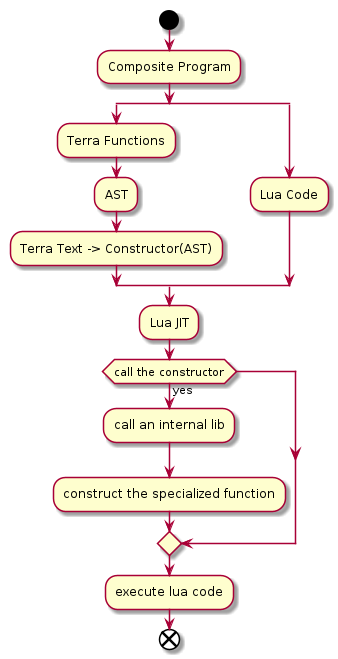
\includegraphics[scale=0.3]{terra.png}
\end{frame}

\begin{frame}[fragile]
	\frametitle{Some Code Examples}
  \begin{lstlisting}
    terra min(a: int, b: int): int
      if a < b then return a
      else return b end
    end
    struct GreyScaleImage {
      data: &float
      N: int
    }
  \end{lstlisting}
\end{frame}

\begin{frame}
	\frametitle{Features}
  \begin{itemize}
  \item Terra entities are all first-class Lua values.\pause
  \item Terra functions will be executed in LLVM JIT.\pause
  \item You can dump Terra functions to an object file(i.e. something.o in Linux) if you like.\pause
  \item Quotation: using brackets($[]$) for escaping and backtick(expressions)/quote keyword(statements) for creating quotation.
  \end{itemize}
\end{frame}

\begin{frame}[fragile]
  \frametitle{Quotation Example}
  \begin{lstlisting}
    local a = 5
    terra sin5()
      return [ math.sin(a) ]
      end
    function addtwo(a,b)
      return `a + b
    end
    local printtwice = quote
      C.printf("hello\n")
      C.printf("hello\n")
    end
  \end{lstlisting}
\end{frame}

\begin{frame}
	\frametitle{It Just Works!}
  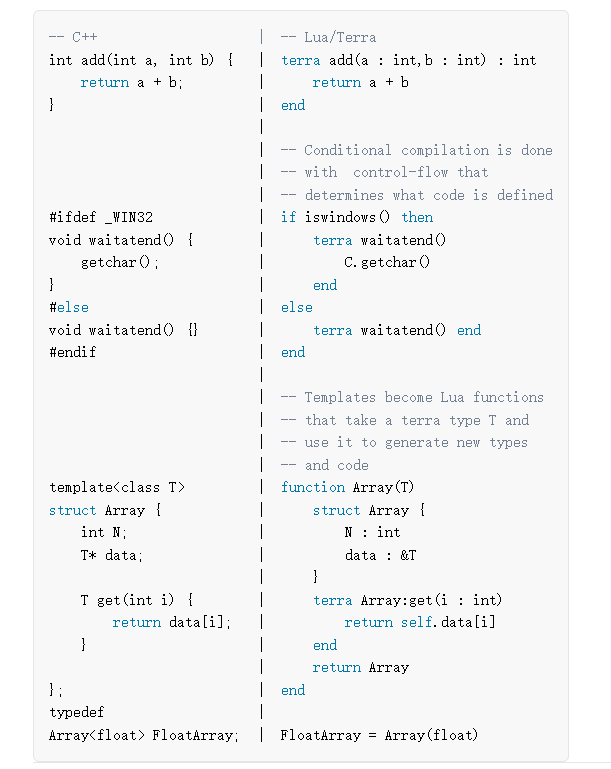
\includegraphics[scale=0.45]{terra2.png}
\end{frame}

\begin{frame}
	\frametitle{It Just Works!}
  \begin{itemize}
  \item Now we can generate code dynamically.\pause
  \item e.g. block the loop nests to make the memory access more friendly to the cache.
  \end{itemize}
\end{frame}

\begin{frame}
	\frametitle{The Formal Calculus: Terra Core}
  \begin{itemize}
  \item For simplicity, Lua := imperative language + first-class functions, Terra := purely functional language\pause
  \item Lua expression: $e$, evaluation of Lua: $\xrightarrow[]{L}$\pause
  \item Terra expression: $\dot{e}$, specialization of Terra: $\xrightarrow[]{S}$\pause
  \item Specialized Terra expression: $\underline{\dot{e}}$, execution of specailized Terra expression: $\xrightarrow[]{T}$
  \end{itemize}
\end{frame}

\begin{frame}
	\frametitle{Terra Core}
  Lua Syntax:
  \newline
  \begin{equation}
    \begin{split}
      e\, ::=\, & b\, |\, \dot{T}\, |\, x\, |\, let\, x\, =\, e\, in\, e\, |\, x\, :=\, e\, |\, e(e)\, |\, fun(x)\{e\}\, |\, tdecl\, | \\ & ter\, e(x:\, e):\, e \{\dot{e}\}\, |\, \backprime \dot{e}\\
      v\, ::=\, & b\, |\, l\, |\, \dot{T}\, |\, <\Gamma, x, e>\, |\, \underline{\dot{e}}\\
      \dot{T} ::=\, & \dot{B}\, |\, \dot{T} \rightarrow \dot{T}
    \end{split} \notag
  \end{equation}
\end{frame}

\begin{frame}
	\frametitle{Terra Core}
  Terra Syntax:
  \newline
  \begin{equation}
    \begin{split}
      \dot{e}\, ::=\, & b\, |\, x\, | \dot{e}(\dot{e}) |\, tlet\, x:\, e\, =\, \dot{e}\, in\, \dot{e}\, |\, [e]\\
      \underline{\dot{e}}\, ::=\, & b\, |\, \underline{\dot{x}}\, | \underline{\dot{e}}(\underline{\dot{e}}) |\, tlet\, \underline{\dot{x}}:\, \dot{T}\, =\, \underline{\dot{e}}\, in\, \underline{\dot{e}}\, |\, l
    \end{split} \notag
  \end{equation}
\end{frame}

\begin{frame}
  \frametitle{Terra Core}
  \begin{equation}
    v\, \Sigma \xrightarrow[]{L} v\, \Sigma \tag{LVAL}
  \end{equation}
  \newline
  \begin{equation}
    \frac{\Sigma = \Gamma, S, F}{x\, \Sigma \xrightarrow[]{L} S(\Gamma{(x)})\, \Sigma}\tag{LVAR}
  \end{equation}
  \newline
  \begin{equation}
    \frac{e_1 \, \Sigma_1 \xrightarrow[]{L} v_1 \, \Sigma_2 \enspace \Sigma_2 = \Gamma, S, F \enspace e_2 \Sigma_2[x \leftarrow v_1] \xrightarrow[]{L} v_2 \Sigma_3}{let \, x = e_1 \, in \, e_2 \, \Sigma \xrightarrow[]{L} v_2(\Sigma_3 \leftarrow \Gamma)} \tag{LLET}
  \end{equation}
  \newline
  \begin{equation}
    \frac{e \, \Sigma \xrightarrow[]{L} v\, \Gamma, S, F \enspace \Gamma{(x)} = a}{x := e \, \Sigma \xrightarrow[]{L} v \, \Gamma, S[a \leftarrow v], F} \tag{LASN}
  \end{equation}
\end{frame}

\begin{frame}
  \frametitle{Terra Core}
	\begin{equation}
    \frac{\Sigma = \Gamma, S, F}{fun(x)\{e\} \, \Sigma \xrightarrow[]{L} <\Gamma, x, e> \, \Sigma} \tag{LFUN}
  \end{equation}
  \newline
  \begin{equation}
    \begin{split}
      e_1 \, \Sigma_1 \xrightarrow[]{L} <\Gamma_1, x, e_3> \enspace e_2 \, \Sigma_2 \xrightarrow[]{L} v_1 \, \Gamma_2, S, F \\
      \frac{a \, fresh \enspace e_3 \, \Gamma_1[x \leftarrow a], S[a \leftarrow v_1], F \xrightarrow[]{L} v_2 \, \Sigma_3}{e_1(e_2) \, \Sigma_1 \xrightarrow[]{L} v_2 \, (\Sigma_3 \leftarrow \Gamma_2)}
    \end{split} \tag{LAPP}
  \end{equation}
  \newline
  \begin{equation}
    \frac{l\, fresh \enspace \Sigma = \Gamma, S, F}{tdecl \Sigma \xrightarrow[]{L} l \, \Gamma, S, F[l \leftarrow \bullet]} \tag{LTDECL}
  \end{equation}
\end{frame}

\begin{frame}
  \frametitle{Terra Core}
	\begin{equation}
    \begin{split}
      & e_1 \, \Sigma_1 \xrightarrow[]{L} l \, \Sigma_2 \enspace e_2 \, \Sigma_2 \xrightarrow[]{L} \dot{T_1} \, \Sigma_3 \enspace e_3 \, \Sigma_3 \xrightarrow[]{L} \dot{T_2} \, \Sigma_4 \\
      & \Sigma_4 = \Gamma_1, S_1, F_1 \enspace \underline{\dot{x}} \, fresh \\
      & \frac{\dot{e} \, \Sigma_4[x \leftarrow \underline{\dot{x}}] \xrightarrow[]{S} \underline{\dot{e}} \, \Gamma_2, S_2, F_2 \enspace F_2(l) = \bullet}{ter \, e_1(x: e_2): e_3\{\dot{e}\} \, \Sigma_1 \xrightarrow[]{L} l \, \Gamma_1, S_2, F_2[l \leftarrow <\underline{\dot{x}}, \dot{T_1}, \dot{T_2}, \underline{\dot{e}}>]}
    \end{split} \tag{LTDEFN}
  \end{equation}
  \newline
  \begin{equation}
    \frac{\dot{e} \, \Sigma_1 \xrightarrow[]{S} \underline{\dot{e}} \, \Sigma_2}{\backprime{\dot{e}} \, \Sigma_1 \xrightarrow[]{L} \underline{\dot{e}} \, \Sigma_2}\tag{LTQUOTE}
  \end{equation}
\end{frame}

\begin{frame}
  \frametitle{Terra Core}
  \begin{equation}
    \begin{split}
      & e_1 \, \Sigma_1 \xrightarrow[]{L} l \, \Sigma_2 \enspace e_2 \, \Sigma_2 \xrightarrow[]{L} b_1 \, \Sigma_3 \\
      & \Sigma_3 = \Gamma, S, F \enspace F(l) = <\underline{\dot{x}}, \dot{T_1}, \dot{T_2}, \underline{\dot{e}}> \enspace b_1 \in \dot{T_1} \\
      & \frac{[\underline{\dot{x}}: \dot{T_1}], [l: \dot{T_1} \rightarrow \dot{T_2}], F_2 \vdash \underline{\dot{e}}: \dot{T_2} \enspace \underline{\dot{e}}[\underline{\dot{x}} \leftarrow b], F \xrightarrow[]{T} b_2}{e_1(e_2) \, \Sigma_1 \xrightarrow[]{L} b_2 \, \Sigma_3}
    \end{split} \tag{LTAPP}
  \end{equation}
\end{frame}

\begin{frame}
	\frametitle{Terra Core}
  \begin{equation}
    b \, \Sigma \xrightarrow[]{S} b \, \Sigma \tag{SBAS}
  \end{equation}
  \newline
  \begin{equation}
    \frac{\dot{e_1} \, \Sigma_1 \xrightarrow[]{S} \underline{\dot{e_1}} \, \Sigma_2 \enspace \dot{e_2} \Sigma_2 \xrightarrow[]{S} \underline{\dot{e_2}} \Sigma_3}{\dot{e_1}(\dot{e_2}) \, \Sigma_1 \xrightarrow[]{S} \underline{\dot{e_1}}(\underline{\dot{e_2}}) \, \Sigma_3} \tag{SAPP}
  \end{equation}
  \newline
  \begin{equation}
    \begin{split}
      & e \, \Sigma_1 \xrightarrow[]{L} \dot{T} \, \Sigma_2 \enspace \dot{e_1} \, \Sigma_2  \xrightarrow[]{S} \underline{\dot{e_1}} \, \Sigma_3 \enspace \underline{\dot{x}} \, fresh \\
      & \frac{\Sigma_3 = \Gamma, S, F \enspace \dot{e_2} \, \Sigma_3[x \leftarrow \underline{\dot{e_2}}] \xrightarrow[]{S} \underline{\dot{e_2}} \, \Sigma_4}{tlet \, x: e = \dot{e_1} \, in \, \dot{e_2} \, \Sigma_1 \xrightarrow[]{S} tlet \, \underline{\dot{x}}: \dot{T} = \underline{\dot{e_1}} \, in \, \underline{\dot{e_2}} \, (\Sigma_4 \leftarrow \Gamma)}
    \end{split} \tag{SLET}
  \end{equation}
\end{frame}

\begin{frame}
	\frametitle{Terra Core}
  \begin{equation}
    \frac{e \, \Sigma_1 \xrightarrow[]{L} \underline{\dot{e}} \Sigma_2}{[e] \, \Sigma_1 \xrightarrow[]{S} \underline{\dot{e}} \, \Sigma_2} \tag{SESC}
  \end{equation}
  \newline
  \begin{equation}
    \frac{[x] \, \Sigma_1 \xrightarrow[]{S} \underline{\dot{e}} \, \Sigma_2}{x \, \Sigma_1 \xrightarrow[]{S} \underline{\dot{e}} \, \Sigma_2} \tag{SVAR}
  \end{equation}
\end{frame}

\begin{frame}
	\frametitle{Terra Core}
  \begin{equation}
    b \, \dot{\Gamma}, F \xrightarrow[]{T} b \tag{TBAS}
  \end{equation}
  \begin{equation}
    l \, \dot{\Gamma}, F \xrightarrow[]{T} l \tag{TFUN}
  \end{equation}
  \begin{equation}
    \underline{\dot{x}} \, \dot{\Gamma}, F \xrightarrow[]{T} \dot{\Gamma}(\underline{\dot{x}}) \tag{TVAR}
  \end{equation}
  \begin{equation}
    \frac{\underline{\dot{e_1}} \, \dot{\Gamma}, F \xrightarrow[]{T} v_1 \enspace \underline{\dot{e_2}} \dot{\Gamma}[\underline{\dot{x}} \leftarrow v_1], F \xrightarrow[]{T} v_2}{tlet \, \underline{\dot{x}}: \dot{T} = \underline{\dot{e_1}} \, in \, \underline{\dot{e_2}} \, \dot{\Gamma}, F \xrightarrow[]{T} v_2} \tag{TLET}
  \end{equation}
  \begin{equation}
    \begin{split}
      & \underline{\dot{e_1}} \, \dot{\Gamma}, F \xrightarrow[]{T} l \enspace \underline{\dot{e_2}} \, \dot{\Gamma}, F \xrightarrow[]{T} v_1 \\
      & \frac{F(l) = <\underline{\dot{x}}, \dot{T_1}, \dot{T_2}, \underline{\dot{e_3}}> \enspace \underline{\dot{e_3}} \, \dot{\Gamma}[\underline{\dot{x}} \leftarrow v_1], F \xrightarrow[]{T} v_2}{\underline{\dot{e_1}}(\underline{\dot{e_2}}) \, \dot{\Gamma}, F \xrightarrow[]{T} v_2}
    \end{split}\tag{TAPP}
  \end{equation}
\end{frame}

\begin{frame}
	\frametitle{Terra Core}
  \begin{itemize}
  \item The typing rules are very simple. Skip.\pause
  \item Let's see the proof.\pause
  \item No proof! :)
  \end{itemize}
\end{frame}

\begin{frame}
  \frametitle{Some Important Designs}
  \begin{itemize}
  \item Use shared lexical environments to reduce the need for escape expressions.\pause
  \item Perform specialization eagerly.\pause
  \item Perform typechecking and linking lazily.\pause
  \item Type Reflection API.
  \end{itemize}
\end{frame}

\begin{frame}
	\frametitle{Why Specialize Eagerly?}
  \begin{equation*}
    \begin{split}
      & let \, x_1\, =\, 0 \\
      & let \, y\, =\, ter\, tdecl(x_2:\, int):\, int\, \{x_1\}\, in \\
      & x_1\, :=\, 1;\, y(0)
    \end{split}
  \end{equation*} \pause
  \newline
  \begin{itemize}
  \item $y(0) = 0$ if we specialize eagerly.\pause
  \item If not, the Terra runtime must depends on the Lua runtime to get correct value of $x_1$.\pause
  \item Or we need to re-compile $y$ when $x_1$ changes.\pause
  \item Requires declaration before using a symbol, which makes recusive function impossible.\pause
  \item Separate the declaration and definition.
  \end{itemize}
\end{frame}

\begin{frame}
	\frametitle{Why Typecheck Lazily?}
  \begin{itemize}
  \item Possible if we use type annotations.\pause
  \item Since a function may have no definition, this may not help.\pause
  \item So no need for type annotations.\pause
  \item Easier to override the default bevavior of a type.
  \end{itemize}
\end{frame}

\begin{frame}[fragile]
	\frametitle{Type Reflection}
  \begin{itemize}
  \item Terra types are first-class in Lua.\pause
  \item Provide methods in Lua(e.g. t:ispointer or t:isstruct).\pause
  \item Use entries table to describe structures' in-memory layout.
  \end{itemize}

  \begin{lstlisting}
    struct Complex {}
    Complex.entries:insert { field = "real",
      type = float }
    Complex.entries:insert { field = "imag",
      type = float }
\end{lstlisting}\pause

  \begin{itemize}
  \item Also the metamethods table: override certain compile-time behaviors(e.g. implicit conversion).
  \end{itemize}
\end{frame}

\begin{frame}
	\frametitle{Evaluation}
  \begin{itemize}
  \item Similar performance to ATLAS, which is written in C and assembly.\pause
  \item Shorter code, easier to read/write/maintain.
  \end{itemize}
\end{frame}

\begin{frame}
	\frametitle{Summary}
  \begin{itemize}
  \item Two-Languages design: Lua + Terra.\pause
  \item Shared lexical scoping.\pause
  \item Seperate Evaluationn: Lua(LuaJIT), Terra(LLVM JIT).\pause
  \item Type Reflection.
  \end{itemize}
\end{frame}

\begin{frame}
	\frametitle{Advantages}
  \begin{itemize}
  \item No need to write C, but the performance is still good.\pause
  \item Generating code dynamically allows us to use runtime information from LuaJIT.\pause
  \item Easy to re-use C/C++ libraries in Lua.\pause
  \end{itemize}
\end{frame}

\begin{frame}
	\frametitle{Shortages}
  \begin{itemize}
  \item Lua is not statically typed.
  \end{itemize}
\end{frame}

\begin{frame}
	\frametitle{Reference}
  \begin{itemize}
  \item Zachary DeVito, James Hegarty, Alex Aiken, Pat Hanrahan, and Jan Vitek. 2013. Terra: A multi-stage language for highperformance computing. In Proceedings of the 34th ACM SIGPLAN Conference on Programming Language Design and Implementation (PLDI’13). ACM, New York, 105–116. DOI:\url{https://doi.org/10.1145/2491956.2462166}
  \item Terra: A low-level counterpart to Lua. \url{https://terralang.org/}
  \end{itemize}
\end{frame}

\end{document}

